% #📘 Chapter3_MultipleAccessScheduling.tex
\chapter{Multiple Access and Scheduling}

\section{Introduction}
Modern cellular networks support simultaneous access for a large number of users. Efficient multiple access techniques and intelligent scheduling algorithms are essential for maximizing throughput and ensuring fairness. This chapter explores various access schemes including FDMA, TDMA, OFDMA, and NOMA, and introduces key scheduling strategies.

\section{Multiple Access Techniques}

\subsection{Frequency Division Multiple Access (FDMA)}
In FDMA, the available frequency spectrum is divided into multiple frequency bands, and each user is assigned a distinct band.

\begin{figure}[H]
    \centering
    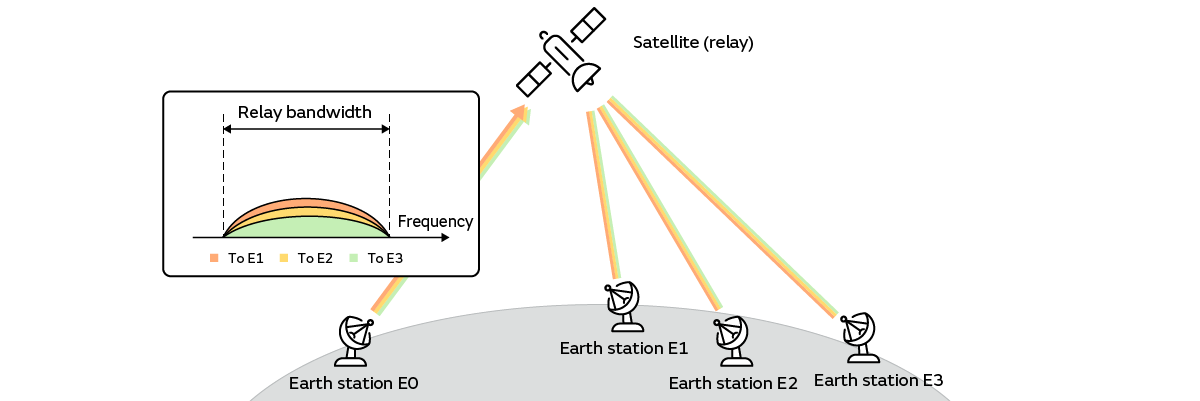
\includegraphics[width=0.85\textwidth]{images/fdma_example.png}
    \caption{FDMA resource allocation example.}
\end{figure}

\subsection{Time Division Multiple Access (TDMA)}
TDMA divides time into slots. Each user is given a dedicated time slot in a cyclic manner.

\begin{figure}[H]
    \centering
    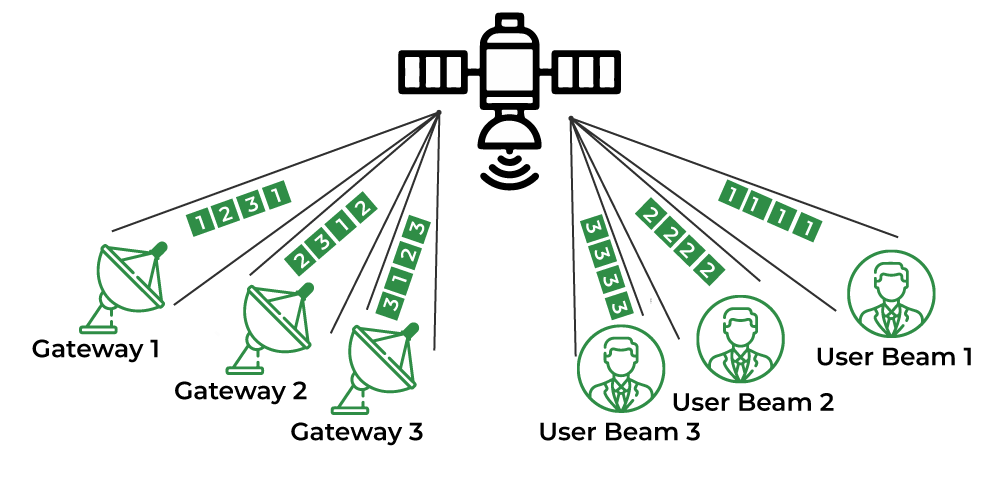
\includegraphics[width=0.85\textwidth]{images/tdma_example.png}
    \caption{TDMA time-slot allocation.}
\end{figure}

\subsection{Orthogonal Frequency Division Multiple Access (OFDMA)}
OFDMA is widely used in 4G and 5G systems. It divides the spectrum into many subcarriers and assigns them orthogonally to users.

\begin{equation}
X_k = \sum_{n=0}^{N-1} x_n e^{-j2\pi kn/N}
\end{equation}

Where:
\begin{itemize}
  \item $X_k$ is the $k$-th subcarrier symbol
  \item $x_n$ is the data on subcarrier $n$
  \item $N$ is the total number of subcarriers
\end{itemize}

\subsection{Non-Orthogonal Multiple Access (NOMA)}
NOMA allows multiple users to share the same time-frequency resources by using power-domain multiplexing and successive interference cancellation (SIC).

\begin{figure}[H]
    \centering
    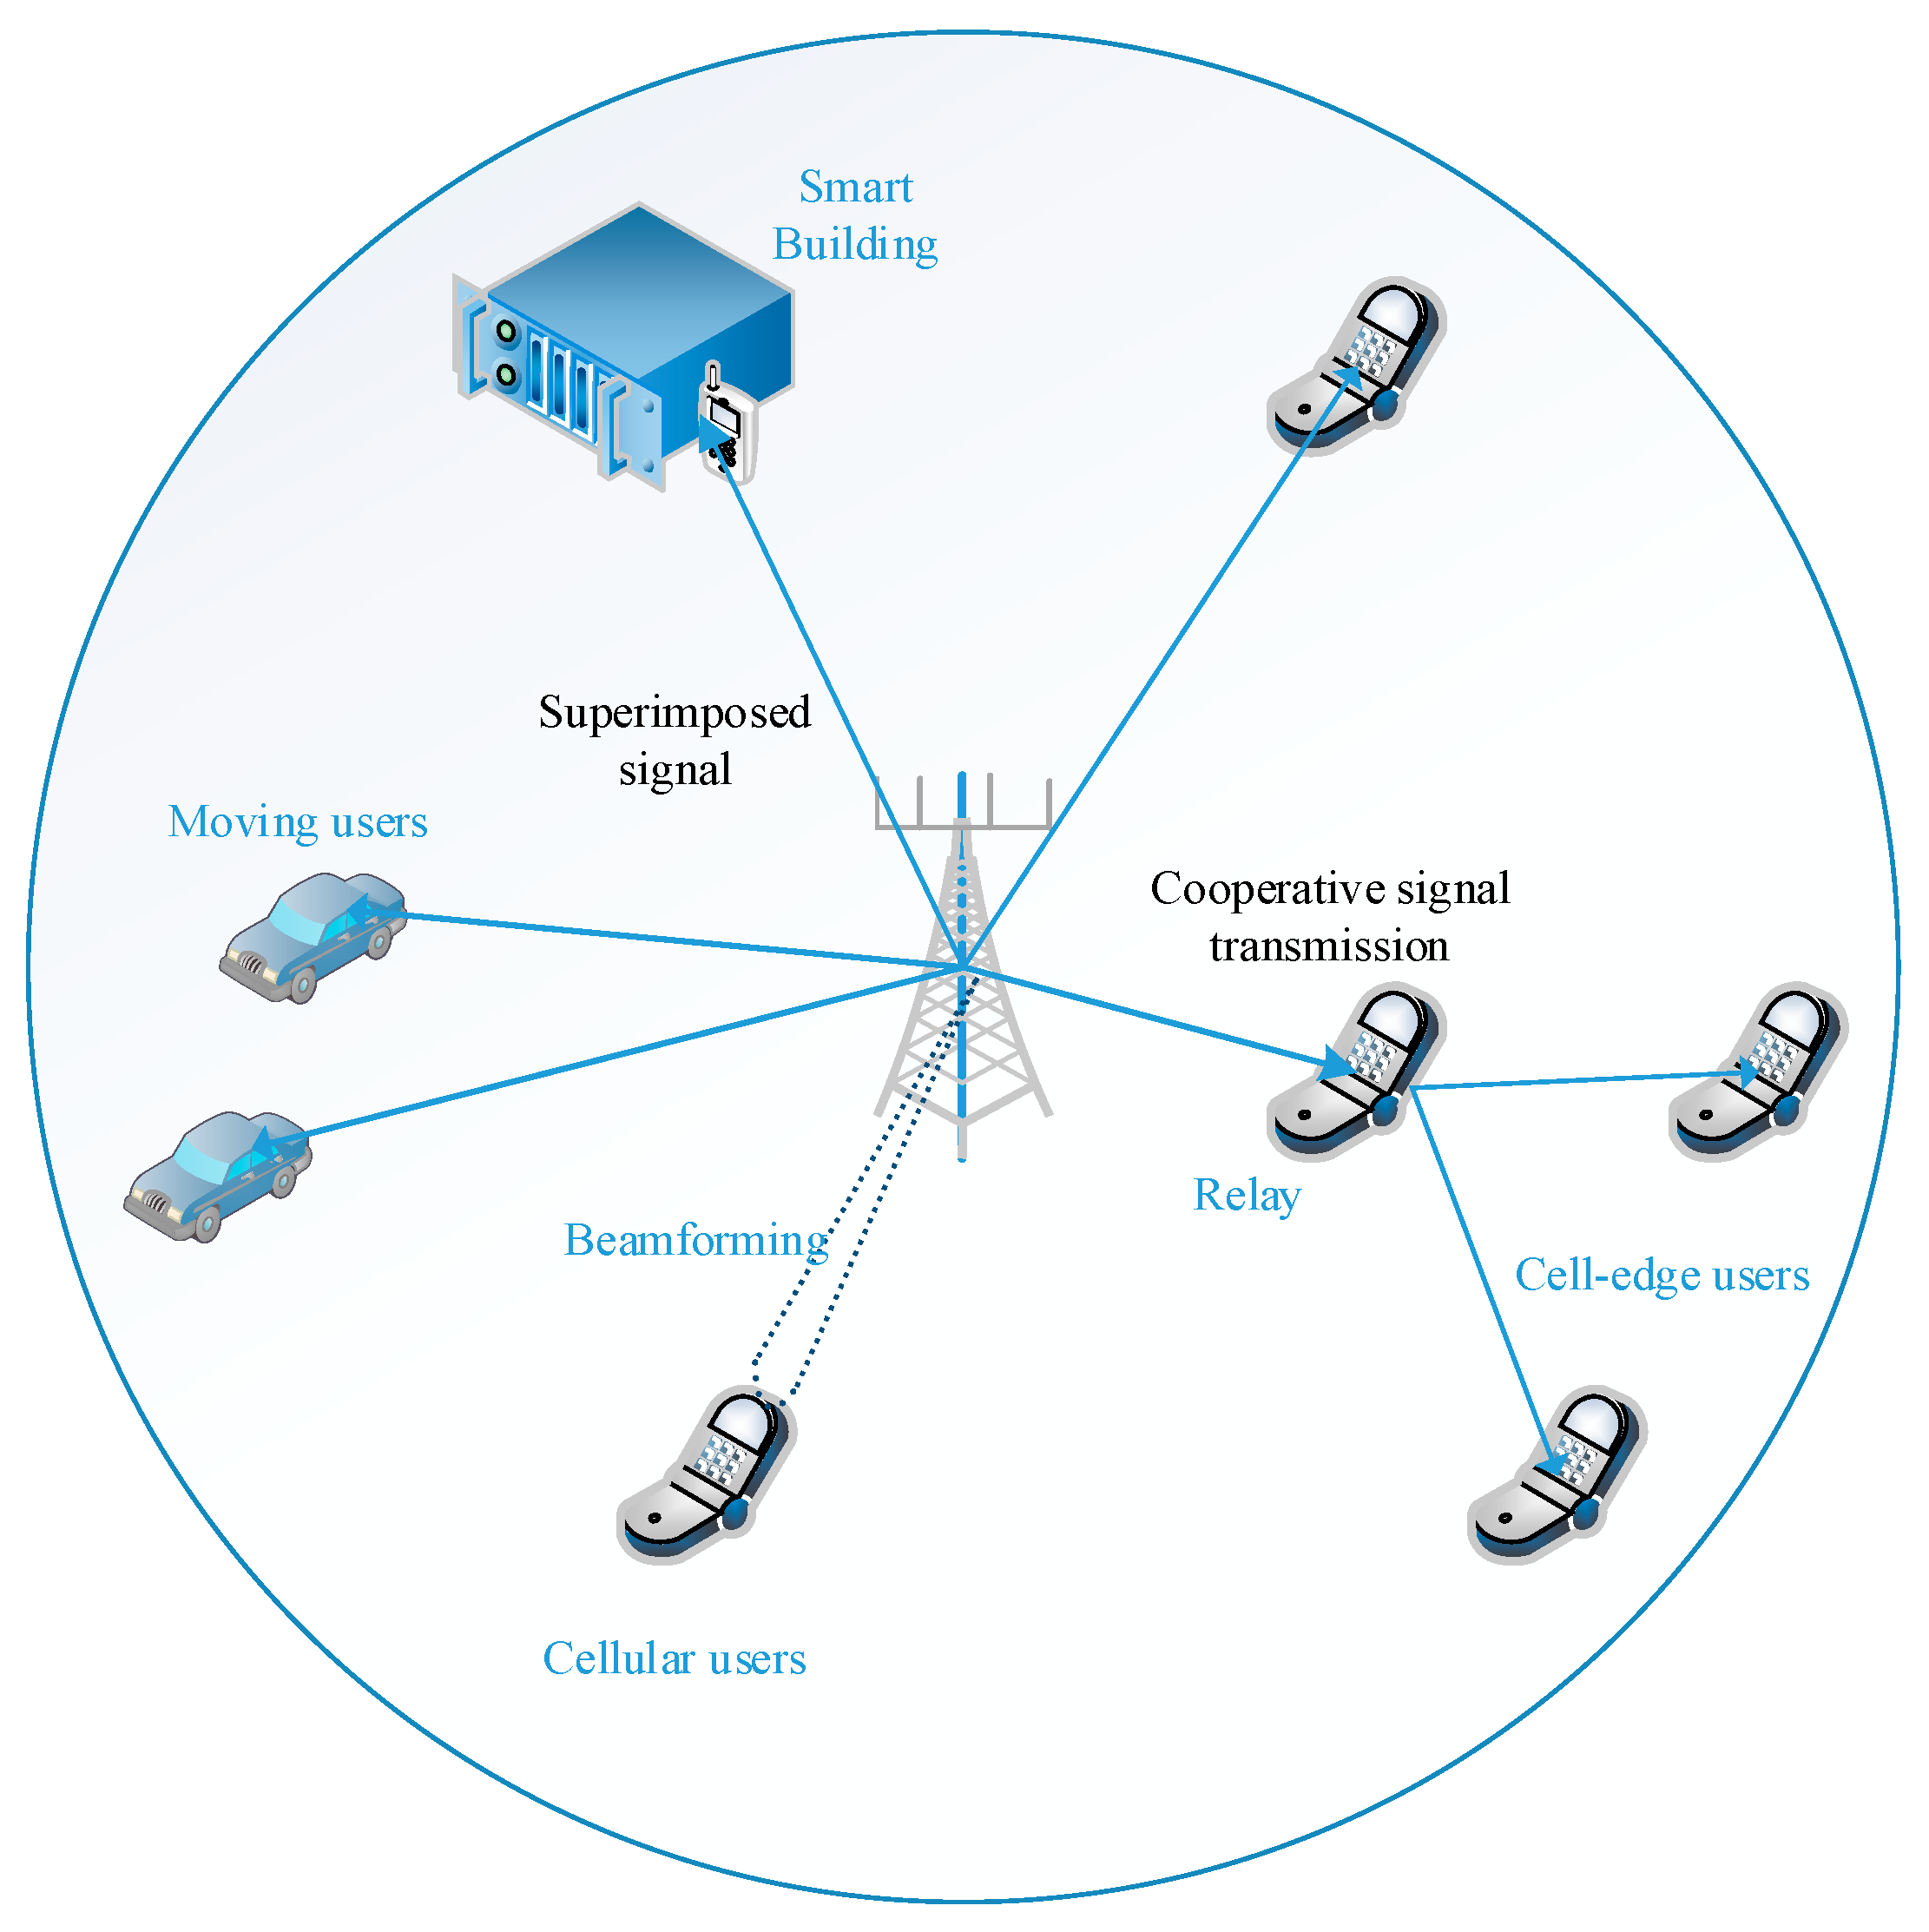
\includegraphics[width=0.75\textwidth]{images/noma_example.png}
    \caption{NOMA with successive interference cancellation.}
\end{figure}

\section{Scheduling Strategies}

\subsection{Round Robin (RR) Scheduler}
This scheduler allocates time slots to users in a cyclic order, ensuring fairness but not necessarily optimizing throughput.

\subsection{Proportional Fair (PF) Scheduler}
PF scheduler attempts to balance fairness and throughput. The metric is defined as:

\begin{equation}
M_i = \frac{R_i(t)}{\bar{R}_i(t)}
\end{equation}

Where:
\begin{itemize}
  \item $R_i(t)$ is the instantaneous rate of user $i$
  \item $\bar{R}_i(t)$ is the historical average rate
\end{itemize}

\section{Comparative Overview}

\begin{table}[H]
\centering
\begin{tabular}{|l|l|l|}
\hline
\textbf{Scheme} & \textbf{Orthogonal} & \textbf{Used In} \\
\hline
FDMA & Yes & 1G \\
TDMA & Yes & 2G \\
OFDMA & Yes & 4G, 5G \\
NOMA & No & 5G, 6G \\
\hline
\end{tabular}
\caption{Comparison of multiple access techniques.}
\end{table}

\section{Conclusion}
Multiple access and scheduling techniques form the backbone of cellular systems. Understanding their principles allows for better network optimization and user experience.

\vspace{1em}
\noindent\textbf{Next:} Appendix section includes hands-on simulations using Jupyter notebooks and Streamlit apps.

